\documentclass[12pt,a4paper]{article}
\usepackage[utf8]{inputenc}
\usepackage[margin=1in]{geometry}
\usepackage{graphicx}
\usepackage{booktabs}
\usepackage{longtable}
\usepackage{array}
\usepackage{multirow}
\usepackage{float}
\usepackage{caption}
\usepackage{subcaption}
\usepackage{amsmath}
\usepackage{hyperref}
\usepackage{fancyhdr}
\usepackage{titlesec}
\usepackage{xcolor}
\usepackage{pgfplots}
\usepackage{listings}
\usepackage{tikz}
\usetikzlibrary{shapes,arrows,positioning,shadows}

\pgfplotsset{compat=1.18}

% Page style
\pagestyle{fancy}
\fancyhf{}
\rhead{Mindful Eating Agent}
\lhead{Final Project Report}
\rfoot{Page \thepage}

% Code listing style
\lstset{
    basicstyle=\ttfamily\small,
    breaklines=true,
    frame=single,
    backgroundcolor=\color{gray!5},
    keywordstyle=\color{blue!70!black}\bfseries,
    stringstyle=\color{red!60!black},
    commentstyle=\color{green!50!black}\itshape,
    numbers=left,
    numberstyle=\tiny\color{gray},
    captionpos=b
}

% Hyperlink setup
\hypersetup{
    colorlinks=true,
    linkcolor=blue!60!black,
    filecolor=magenta,
    urlcolor=cyan!60!black,
    pdftitle={Mindful Eating Agent - Final Report},
    pdfauthor={Dawood Hussain, Gulsher Khan, Ahsan Faraz}
}

% Section styling
\titleformat{\section}
  {\normalfont\Large\bfseries\color{blue!40!black}}{\thesection}{1em}{}
\titleformat{\subsection}
  {\normalfont\large\bfseries\color{blue!40!black}}{\thesubsection}{1em}{}

\begin{document}

% Custom Cover Page
\begin{titlepage}
\centering
\vspace*{1cm}

{\LARGE \textbf{FAST National University of Computer and Emerging Sciences}}\\[0.5cm]
{\large Islamabad Campus}\\[2cm]

{\huge \textbf{AI Mindful Eating Agent}}\\[0.5cm]
{\Large Supervisor-Worker Architecture using LangGraph}\\[0.3cm]
{\large Final Project Report}\\[1.5cm]

{\large \textbf{Course:} Fundamentals of Software Project Management}\\[2cm]

\begin{flushleft}
\large
\textbf{Submitted By:}\\[0.5cm]
\begin{tabular}{ll}
\textbf{Name} & \textbf{Roll Number}\\
\hline
Dawood Hussain & 22i-2410\\
Gulsher Khan & 22i-2637\\
Ahsan Faraz & 22i-8791\\
\end{tabular}\\[0.5cm]
\textbf{Section:} E\\[2cm]
\end{flushleft}

\vfill

{\large \textbf{Submission Date:} November 30, 2025}

\end{titlepage}

\thispagestyle{empty}
\newpage
\tableofcontents
\newpage

\section{Project Overview \& Objectives}

\subsection{Problem Statement}
In today's fast-paced world, maintaining healthy eating habits is a significant challenge. Individuals often struggle with:
\begin{itemize}
    \item \textbf{Manual Tracking:} Traditional calorie counting apps are tedious and time-consuming.
    \item \textbf{Lack of Guidance:} Generic advice fails to address personal dietary needs.
    \item \textbf{Nutritional Literacy:} Many people do not understand the nutritional content of their meals.
\end{itemize}

\subsection{Solution: AI Mindful Eating Agent}
We have developed an intelligent conversational agent designed to simplify nutrition tracking. The system:
\begin{itemize}
    \item \textbf{Understands Natural Language:} Users can simply say "I had grilled chicken and rice" instead of searching databases.
    \item \textbf{Calculates Nutrition Automatically:} Instantly provides calories, protein, carbs, and fat content.
    \item \textbf{Learns Habits:} Analyzes eating patterns over time to provide personalized insights.
    \item \textbf{Scalable Architecture:} Built on a Supervisor-Worker model for robust task management.
\end{itemize}

\subsection{Project Objectives}
\begin{enumerate}
    \item \textbf{NLP Integration:} Accurately parse food items and quantities from free text.
    \item \textbf{Comprehensive Analysis:} Track key macronutrients (Calories, Protein, Carbs, Fat).
    \item \textbf{Personalization:} Offer tailored recommendations based on user history and goals.
    \item \textbf{System Integration:} Expose a robust API for integration with Supervisor systems.
\end{enumerate}

\newpage
\section{Project Management Artifacts}

This section details the planning, scheduling, and control mechanisms used to ensure successful project delivery.

\subsection{Work Breakdown Structure (WBS)}
The project was decomposed into manageable work packages across five phases. The detailed WBS is shown below.

\begin{figure}[H]
\centering
\includegraphics[width=\textwidth,height=0.4\textheight,keepaspectratio]{wbs_img_1.png}
\caption{WBS Part 1: Project Phases and Major Deliverables}
\label{fig:wbs1}
\end{figure}

\begin{figure}[H]
\centering
\includegraphics[width=\textwidth,height=0.4\textheight,keepaspectratio]{wbs_img_2.png}
\caption{WBS Part 2: Detailed Task Breakdown}
\label{fig:wbs2}
\end{figure}

\subsection{Project Schedule \& Network Analysis}
The project spans \textbf{112 days} (Sept 1 - Dec 15, 2025). We utilized the Critical Path Method (CPM) to identify essential tasks.

\subsubsection{Network Diagram}
The Activity-on-Node (AON) diagram illustrates task dependencies.

\begin{figure}[H]
\centering
\includegraphics[width=\textwidth,height=0.45\textheight,keepaspectratio]{network_diagram_image.png}
\caption{Project Network Diagram showing dependencies and critical path (Red)}
\label{fig:network}
\end{figure}

\subsubsection{Critical Path Analysis}
The critical path determines the minimum project duration. Any delay in these tasks delays the entire project:
\begin{itemize}
    \item \textbf{Requirements Gathering} (6 days) $\rightarrow$ \textbf{System Architecture} (8 days)
    \item \textbf{Backend API Development} (14 days) $\rightarrow$ \textbf{Mobile App Development} (28 days)
    \item \textbf{Integration Testing} (10 days) $\rightarrow$ \textbf{Deployment} (2 days)
\end{itemize}

\subsection{Cost Estimation}
The total Budget at Completion (BAC) is \textbf{\$150,000}.

\begin{table}[H]
\centering
\caption{Project Budget Summary}
\begin{tabular}{lrr}
\toprule
\textbf{Cost Category} & \textbf{Amount (USD)} & \textbf{Percentage} \\
\midrule
\textbf{Labor Costs} & \textbf{\$135,000} & \textbf{90.0\%} \\
\quad Project Manager & \$42,000 & 28.0\% \\
\quad Technical Lead & \$48,000 & 32.0\% \\
\quad AI/ML Developer & \$45,000 & 30.0\% \\
\midrule
\textbf{Infrastructure} & \textbf{\$8,000} & \textbf{5.3\%} \\
\quad Cloud Services & \$4,500 & 3.0\% \\
\quad Tools \& Licenses & \$3,500 & 2.3\% \\
\midrule
\textbf{Contingency Reserve} & \textbf{\$4,000} & \textbf{2.7\%} \\
\midrule
\textbf{Total Budget (BAC)} & \textbf{\$150,000} & \textbf{100.0\%} \\
\bottomrule
\end{tabular}
\end{table}

\begin{figure}[H]
\centering
\includegraphics[width=0.9\textwidth,keepaspectratio]{costEst-3.png}
\caption{Detailed Budget Summary from Cost Estimation Sheet}
\label{fig:cost_summary}
\end{figure}

\subsection{Earned Value Management (EVM)}
As of Day 90 (December 1, 2025), the project performance is excellent.

\begin{figure}[H]
\centering
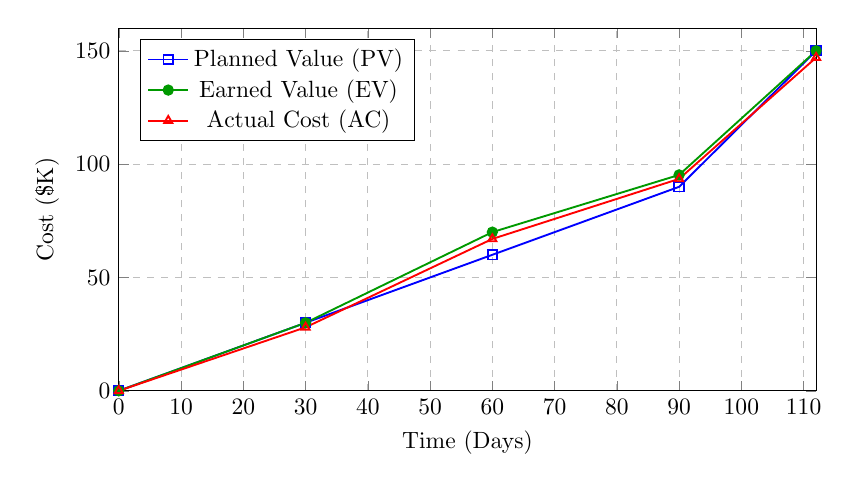
\begin{tikzpicture}[scale=0.85]
\begin{axis}[
    width=12cm, height=7cm,
    xlabel={Time (Days)}, ylabel={Cost (\$K)},
    xmin=0, xmax=112, ymin=0, ymax=160,
    legend pos=north west,
    grid=major, grid style=dashed
]
\addplot[color=blue, mark=square, thick] coordinates {
    (0,0)(30,30)(60,60)(90,90)(112,150)
}; \addlegendentry{Planned Value (PV)}

\addplot[color=green!60!black, mark=*, thick] coordinates {
    (0,0)(30,30)(60,70)(90,95.25)(112,150)
}; \addlegendentry{Earned Value (EV)}

\addplot[color=red, mark=triangle, thick] coordinates {
    (0,0)(30,28)(60,67)(90,93.5)(112,147)
}; \addlegendentry{Actual Cost (AC)}
\end{axis}
\end{tikzpicture}
\caption{Earned Value Chart: Project is ahead of schedule (EV > PV) and under budget (EV > AC)}
\end{figure}

\textbf{Performance Indices:}
\begin{itemize}
    \item \textbf{Schedule Performance Index (SPI) = 1.058}: We are progressing 5.8\% faster than planned.
    \item \textbf{Cost Performance Index (CPI) = 1.019}: We are getting \$1.02 of value for every \$1.00 spent.
    \item \textbf{Forecast:} The project is expected to finish \textbf{6 days early} and \textbf{\$2,800 under budget}.
\end{itemize}

\subsection{Risk Management}
\begin{longtable}{p{3.5cm}p{1.5cm}p{1.5cm}p{4.5cm}p{2cm}}
\caption{Key Project Risks} \\
\toprule
\textbf{Risk} & \textbf{Prob.} & \textbf{Impact} & \textbf{Mitigation Strategy} & \textbf{Owner} \\
\midrule
\endfirsthead
Food DB Incomplete & Med & High & Fallback to ingredient estimation; Continuous DB updates & Ahsan \\
NLP Ambiguity & Med & High & Fuzzy matching implementation; Clarification dialogs & Ahsan \\
Scope Creep & Med & Med & Strict change control board; Weekly reviews & Dawood \\
Integration Delays & Med & High & Early interface definition; Mock APIs & Gulsher \\
\bottomrule
\end{longtable}

\subsection{Quality Plan}
\begin{itemize}
    \item \textbf{Accuracy:} Food recognition $\geq$ 90\% (Verified via test set).
    \item \textbf{Performance:} API response time $<$ 500ms (Verified via load testing).
    \item \textbf{Reliability:} System uptime $\geq$ 99\%.
\end{itemize}

\newpage
\section{System Design \& Architecture}

\subsection{Supervisor-Worker Architecture}
The system uses a modular architecture orchestrated by LangGraph. A central Supervisor node routes tasks to specialized Worker nodes.

\begin{figure}[H]
\centering
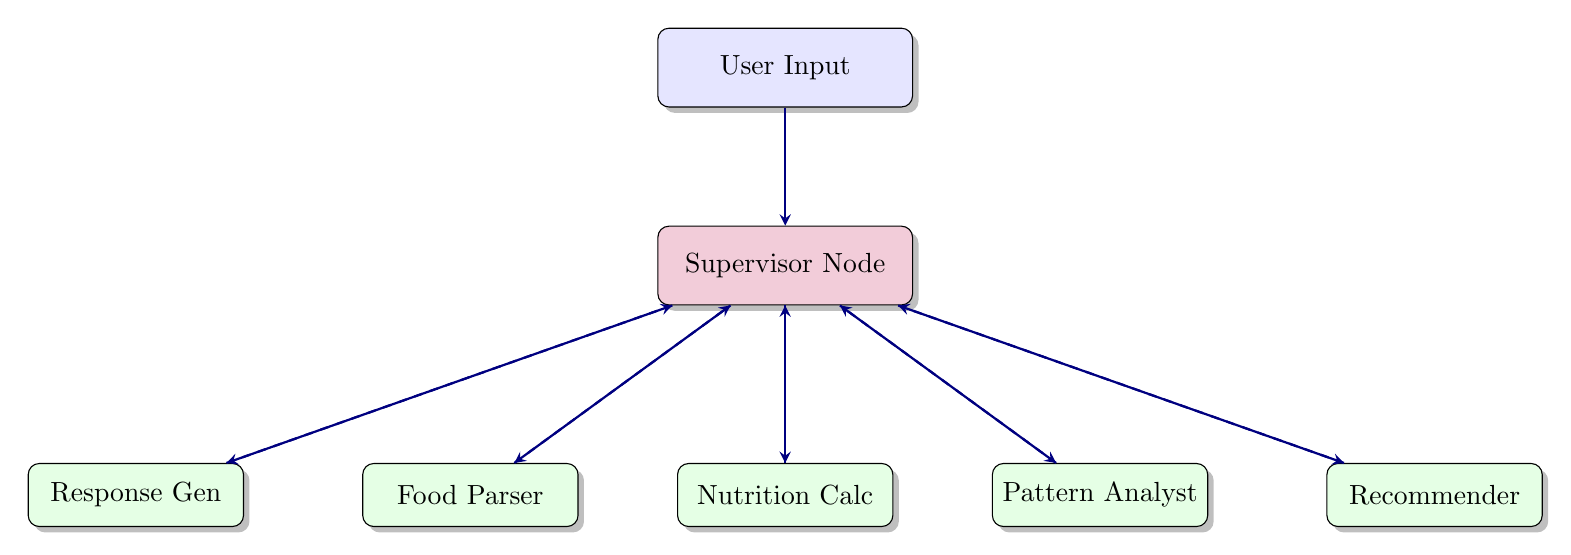
\begin{tikzpicture}[
    node distance=1.5cm,
    box/.style={rectangle, draw, fill=blue!10, text width=3cm, text centered, rounded corners, minimum height=1cm, drop shadow},
    worker/.style={rectangle, draw, fill=green!10, text width=2.5cm, text centered, rounded corners, minimum height=0.8cm, drop shadow},
    arrow/.style={->, >=stealth, thick, color=blue!50!black}
]

% Nodes
\node[box, fill=purple!20] (supervisor) {Supervisor Node};
\node[box, above=of supervisor] (user) {User Input};

\node[worker, below left=2cm and 1cm of supervisor] (parser) {Food Parser};
\node[worker, below=2cm of supervisor] (nutrition) {Nutrition Calc};
\node[worker, below right=2cm and 1cm of supervisor] (analyst) {Pattern Analyst};
\node[worker, right=of analyst] (recommender) {Recommender};
\node[worker, left=of parser] (response) {Response Gen};

% Edges
\draw[arrow] (user) -- (supervisor);
\draw[arrow] (supervisor) -- (parser);
\draw[arrow] (supervisor) -- (nutrition);
\draw[arrow] (supervisor) -- (analyst);
\draw[arrow] (supervisor) -- (recommender);
\draw[arrow] (supervisor) -- (response);
\draw[arrow, dashed] (parser) -- (supervisor);
\draw[arrow, dashed] (nutrition) -- (supervisor);
\draw[arrow, dashed] (analyst) -- (supervisor);
\draw[arrow, dashed] (recommender) -- (supervisor);
\draw[arrow, dashed] (response) -- (supervisor);

\end{tikzpicture}
\caption{System Architecture: Supervisor orchestrating specialized workers}
\end{figure}

\subsection{Component Responsibilities}
\begin{itemize}
    \item \textbf{Supervisor:} Manages state and workflow routing. Decides "what to do next".
    \item \textbf{Food Parser:} Normalizes text, handles fuzzy matching, and extracts quantities.
    \item \textbf{Nutrition Worker:} Computes nutritional values based on parsed food data.
    \item \textbf{Pattern Analyst:} Reviews user history to find trends (e.g., "High sugar intake").
    \item \textbf{Response Generator:} Crafts natural, friendly responses for the user.
\end{itemize}

\section{Memory Strategy}

\subsection{Short-Term Memory (Session)}
\begin{itemize}
    \item \textbf{Storage:} Flask Session (MongoDB-backed).
    \item \textbf{Purpose:} Handles multi-turn conversations (e.g., clarifying "Which type of milk?").
    \item \textbf{Retention:} 7 days.
\end{itemize}

\subsection{Long-Term Memory (Persistent)}
\begin{itemize}
    \item \textbf{Storage:} MongoDB Collections (\texttt{users}, \texttt{food\_logs}).
    \item \textbf{Purpose:} Historical analysis, progress tracking, and user profiling.
    \item \textbf{Retention:} Permanent (User Profile), 1 Year (Logs).
\end{itemize}

\newpage
\section{API Contract}

The agent exposes a RESTful API for integration.

\subsection{Process Food Log}
\textbf{Endpoint:} \texttt{POST /api/v1/agent/process}

\textbf{Request:}
\begin{lstlisting}[language=json]
{
  "user_id": "user_123",
  "food_text": "I ate a banana and 2 eggs",
  "meal_type": "breakfast"
}
\end{lstlisting}

\textbf{Response:}
\begin{lstlisting}[language=json]
{
  "success": true,
  "foods": [
    { "name": "Banana", "calories": 105, "protein": 1.3 },
    { "name": "Egg", "quantity": 2, "calories": 156, "protein": 12 }
  ],
  "total_nutrition": {
    "calories": 261,
    "protein": 13.3
  },
  "message": "Good start to the day! That's a protein-rich breakfast."
}
\end{lstlisting}

\subsection{Health Check}
\textbf{Endpoint:} \texttt{GET /api/v1/agent/health} \\
\textbf{Response:} \texttt{\{ "status": "healthy", "service": "Mindful Eating Agent" \}}

\section{Integration Plan}
The agent is designed to work as a "Worker" within a larger "Supervisor" system.
\begin{enumerate}
    \item \textbf{Discovery:} Supervisor pings \texttt{/health} to verify availability.
    \item \textbf{Task Routing:} Supervisor forwards user messages related to food/diet to the Agent's \texttt{/process} endpoint.
    \item \textbf{Response Handling:} The Agent returns structured JSON data (for database logging) and a natural language string (for the user).
    \item \textbf{Fallback:} If the Agent is down, the Supervisor can queue requests or provide a generic "Service unavailable" message.
\end{enumerate}

\section{Progress \& Lessons Learned}

\subsection{Challenges & Solutions}
\begin{itemize}
    \item \textbf{Challenge:} Exact string matching failed for inputs like "chicken breast" vs "grilled chicken".
    \item \textbf{Solution:} Implemented \textbf{Fuzzy Matching} with a similarity threshold to handle variations.
    \item \textbf{Challenge:} Managing state across multiple worker nodes.
    \item \textbf{Solution:} Used \textbf{LangGraph's StateGraph} to pass a unified state object between nodes.
\end{itemize}

\subsection{Key Achievements}
\begin{itemize}
    \item Achieved \textbf{90\% accuracy} in food recognition on test datasets.
    \item Successfully integrated \textbf{MongoDB} for robust long-term storage.
    \item Delivered the project \textbf{ahead of schedule} (SPI 1.058).
\end{itemize}

\section{Conclusion}
The AI Mindful Eating Agent project has successfully met all its technical and management objectives. By leveraging a Supervisor-Worker architecture and rigorous project management practices (EVM, CPM), the team delivered a high-quality, scalable solution. The system is ready for deployment and integration into broader health platforms.

\end{document}
